% vim: set spell
% vim: spelllang=en
\PassOptionsToPackage{unicode}{hyperref}
\documentclass[aspectratio=1610, 9pt]{beamer}

\usetheme{vertex}

\unimathsetup{math-style=ISO, bold-style=ISO, nabla=upright, partial=upright}


\setmathfont{XITS Math}[range={cal, bfcal}]

\usepackage[main=german, english]{babel}
\usepackage[autostyle]{csquotes}

\usepackage{mathtools}

\usepackage{xcolor}

\usepackage{tcolorbox}
\usepackage[]{siunitx}
\setmathfont{Fira Math}
\AtBeginDocument{\sisetup{math-rm=\mathrm,math-micro=μ}}

\usepackage{graphicx}
\usepackage{tikz}
\usepackage{calc}

% \usepackage{biblatex}

\usepackage{hyperref}
\usepackage{bookmark}

\usepackage{xparse}
\usepackage{expl3}

\NewDocumentCommand \TT {} {\ensuremath{\operatorname{TT}}}
\NewDocumentCommand \TAI {} {\ensuremath{\operatorname{TAI}}}
\NewDocumentCommand \UT {} {\ensuremath{\operatorname{UT1}}}
\NewDocumentCommand \UTC {} {\ensuremath{\operatorname{UTC}}}

\RenewDocumentCommand \d {m} {\TextOrMath{\textd{#1}}{\mathinner{\symup{d}#1}}}

\NewDocumentCommand \heading {m} {{%
  \textcolor{vertexDarkRed}{\bfseries\large #1}
  \par\medskip%
}}

\DeclareSIUnit\arcsecond{as}

\usepackage{tikz-3dplot}


\title{Celestial Coordinates}%

\author[M. Nöthe]{Maximilian Nöthe}
\date[2020-10-09]{Group Seminar 2020-10-09}
\institute[E5b]{
\includegraphics[height=0.1\textheight]{logos/e5b.pdf}}

\begin{document}

\maketitle

\bumper{Where do I need to point my telescope to observe source X?}

\begin{frame}[c]{Overview}
 \tableofcontents
\end{frame}


\bumper{Equatorial Coordinates / ICRS}
\section{Equatorial Coordinates / ICRS}
\begin{frame}[t]{Equatorial Coordinates}
  \centering
  \tdplotsetmaincoords{70}{20}
  \begin{tikzpicture}[tdplot_main_coords, scale=1.5]
    \coordinate (vernal) at (0, -4, 0);
    \coordinate (origin) at (0, 0, 0);
    \node[anchor=center, rotate=-22] at (0, 0, 0) {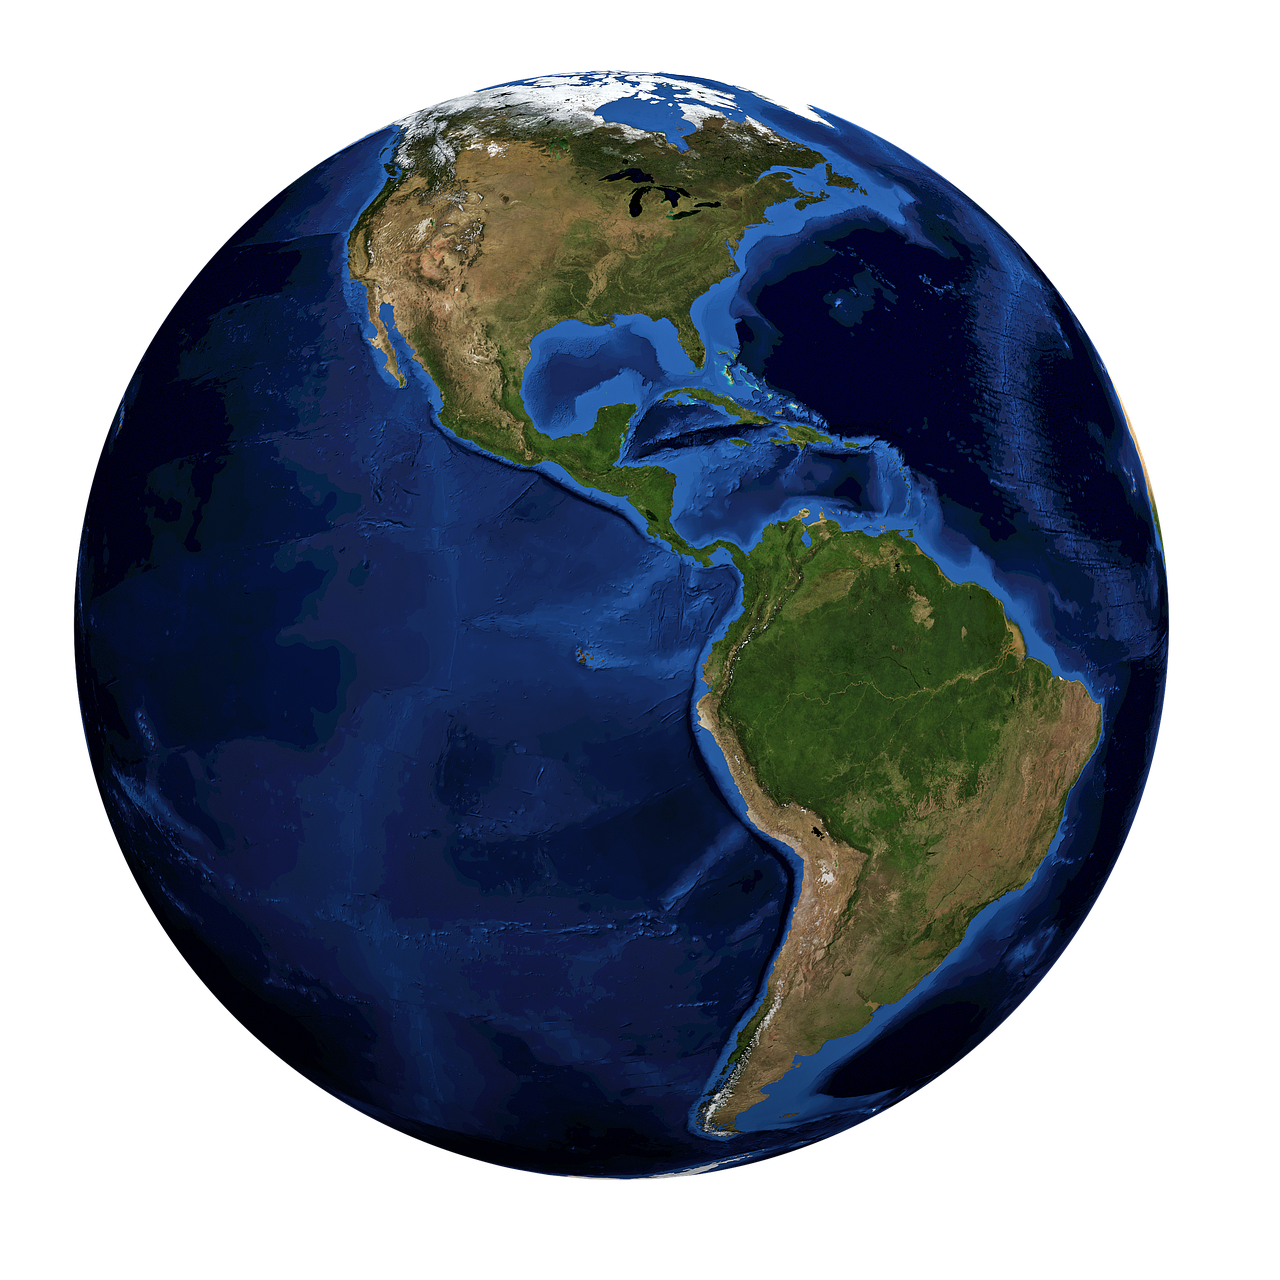
\includegraphics[height=2cm]{images/globe.png}};

    \tdplotdrawarc[thick, color=vertexDarkGrey]{(0, 0, 0)}{4}{0}{360}{}{};

    \tdplotsetrotatedcoords{0}{22}{0}
    \tdplotdrawarc[thick, color=vertexDarkRed, tdplot_rotated_coords]{(0, 0, 0)}{4}{0}{360}{}{};

    % coordinates
    \tdplotdrawarc[thick, color=blue!80!black, tdplot_rotated_coords, ->]{(0, 0, 0)}{4}{-90}{-70}{below, rotate=-22}{\hspace{2em}right ascension};
    \tdplotsetrotatedcoords{0}{22}{0}
    \tdplotsetrotatedthetaplanecoords{90}
    \tdplotdrawarc[thick, color=blue!80!black, tdplot_rotated_coords, ->]{(0, 0, 0)}{4}{-90}{-70}{rotate=68, above}{declination};

    \tdplotsetrotatedcoords{0}{22}{0}
    \node[above right, tdplot_rotated_coords, vertexDarkRed] at (4, 0, 0) {\hspace{2em}Equator};

    \node[above right] at (0, -4, 0) {\hspace{2em}Vernal Equinox};
    \node[above right] at (0, 4, 0) {Autumnal Equinox};
    \node[below right] at (4, 0, 0) {Ecliptic};

    \tdplotsetrotatedcoordsorigin{(vernal)}
    \tdplotsetrotatedcoords{0}{22}{0}
    \tdplotsetrotatedthetaplanecoords{0}
    \tdplotdrawarc[thick, color=vertexDarkRed, tdplot_rotated_coords]{(0, 0, 0)}{1}{65}{87}{right}{obliquity$\color{vertexDarkRed}{} \approx \ang{23}$};

    \tdplotsetrotatedcoords{0}{22}{0}
    \tdplotsetrotatedcoordsorigin{(origin)}
    \draw[vertexDarkRed, tdplot_rotated_coords, thick,->] (0,-0.5,0) -- (0,-4.5,0) node[anchor=north west]{$x$};
    \draw[vertexDarkRed, tdplot_rotated_coords, thick,->] (0.5,0,0) -- (4.5,0,0) node[anchor=north east]{$y$};
    \draw[vertexDarkRed, tdplot_rotated_coords, thick,->] (0,0,0.55) -- (0,0,2.5) node[anchor=north west]{$z$};
    % \node[vertexDarkRed, tdplot_rotated_coords, above] at (0, 0, 2.5) {Earth Rotation Axis};

  \end{tikzpicture}

  \raggedright
\end{frame}

\begin{frame}[c]{International Celestial Reference System / Frame}

  \begin{description}
    \item[Historically] Equatorial coordinates need a reference time for the equinox position
    \item[Modern] The International Celestial Reference Systems defined by VLBI radio sources
  \end{description}

  \begin{itemize}
    \item Origin at Solarsystem Barycenter
    \item Space-fixed, non-rotating
    \item Implemented by reference Frames, catalogues of reference sources with reference coordinates
    \item For backwards compatibility: very close to J2000 equatorial coordinates (\SI{0.02}{\arcsecond})
  \end{itemize}

\end{frame}



\begin{frame}[c]{Full Transformation Equation}
  \Huge
  \begin{equation*}
    \symbf{x}_\text{sky} = \symbf{P} \cdot \symbf{N} \cdot \symbf{T} \cdot \symbf{W} \cdot \symbf{x}_\text{earth}
  \end{equation*}

  \large
  \begin{description}
    \item[$\symbf{P}$] Precession
    \item[$\symbf{N}$] Nutation
    \item[$\symbf{T}$] Earth's rotation
    \item[$\symbf{W}$] Polar Motion
  \end{description}
\end{frame}

\section{Time}
\bumper{Time}

\begin{frame}{The Two Concepts of Time}
  \begin{columns}[t, onlytextwidth]
    \begin{column}{0.475\textwidth}
      \begin{center}
        \heading{Earth's Orientation}
        \only<1>{%
          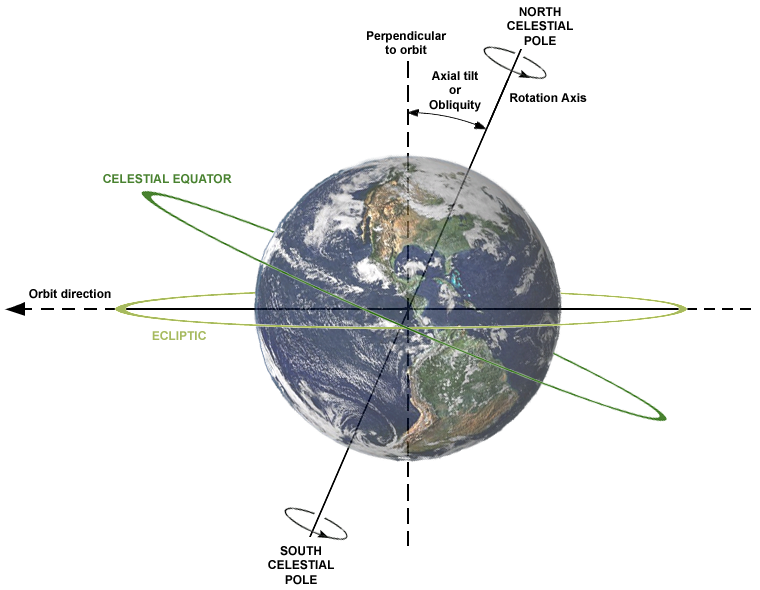
\includegraphics[height=3.5cm]{images/AxialTiltObliquity.png}\\[-1.2\baselineskip]
          \hspace{2.5cm}{\small[Dna-Dennis]}
        }%
        \only<2->{%
          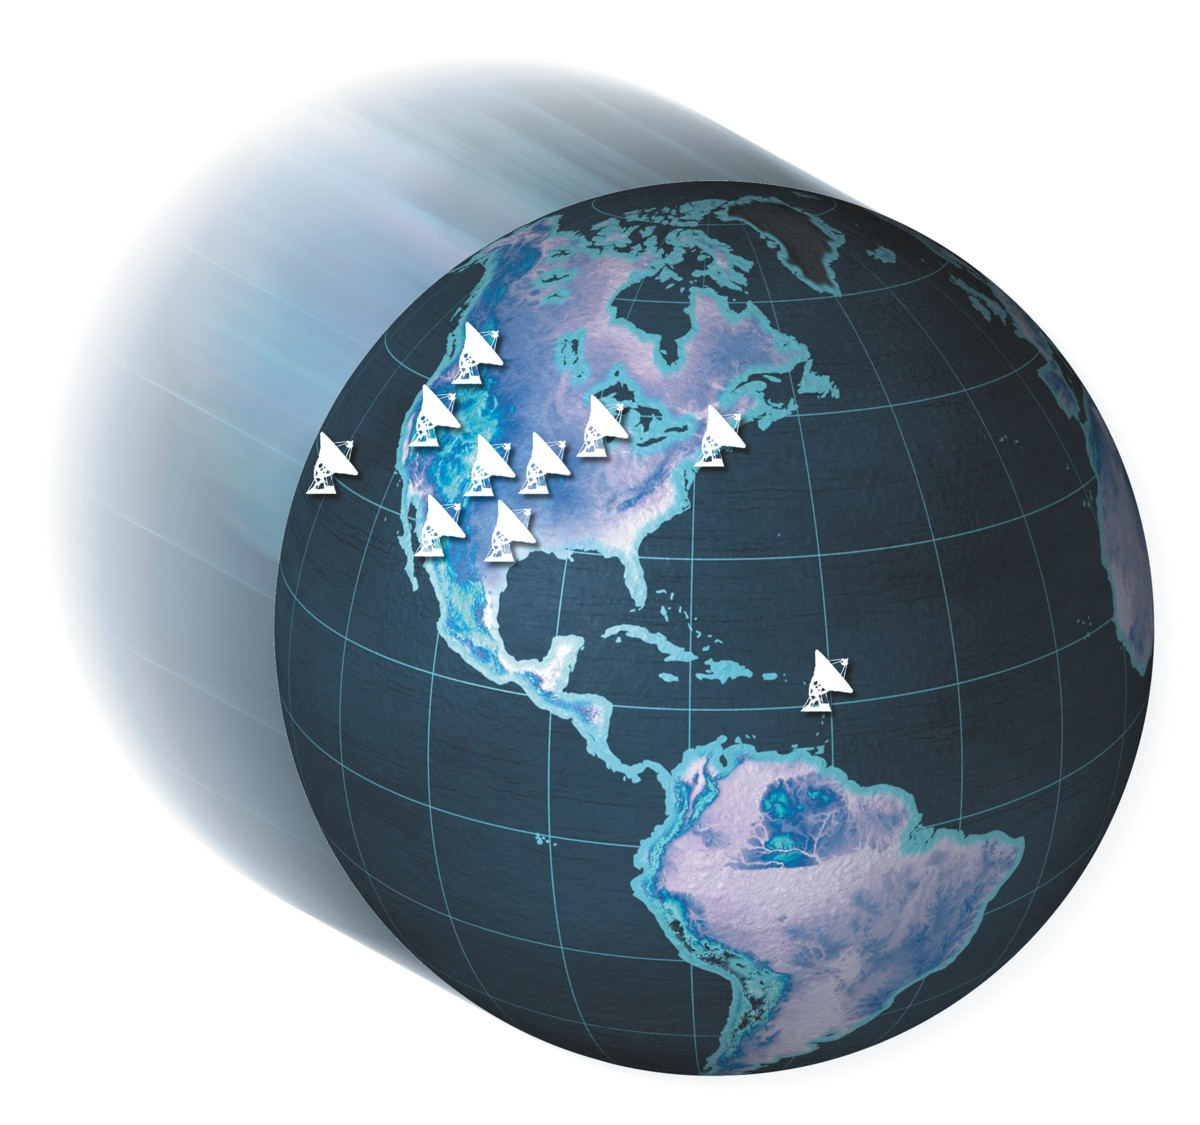
\includegraphics[height=3.5cm]{images/vlba.jpeg}\\[-1.2\baselineskip]
          \hspace{-3.5cm}{\small[NASA]}
        }%
      \end{center}

      \begin{itemize}
        \item The historical concept
        \item Base of calendars $⇒ $ leap years
      \end{itemize}
    \end{column}
    \begin{column}{0.525\textwidth}
      \onslide<3->{
        \begin{center}
          \heading{Linear Time}
          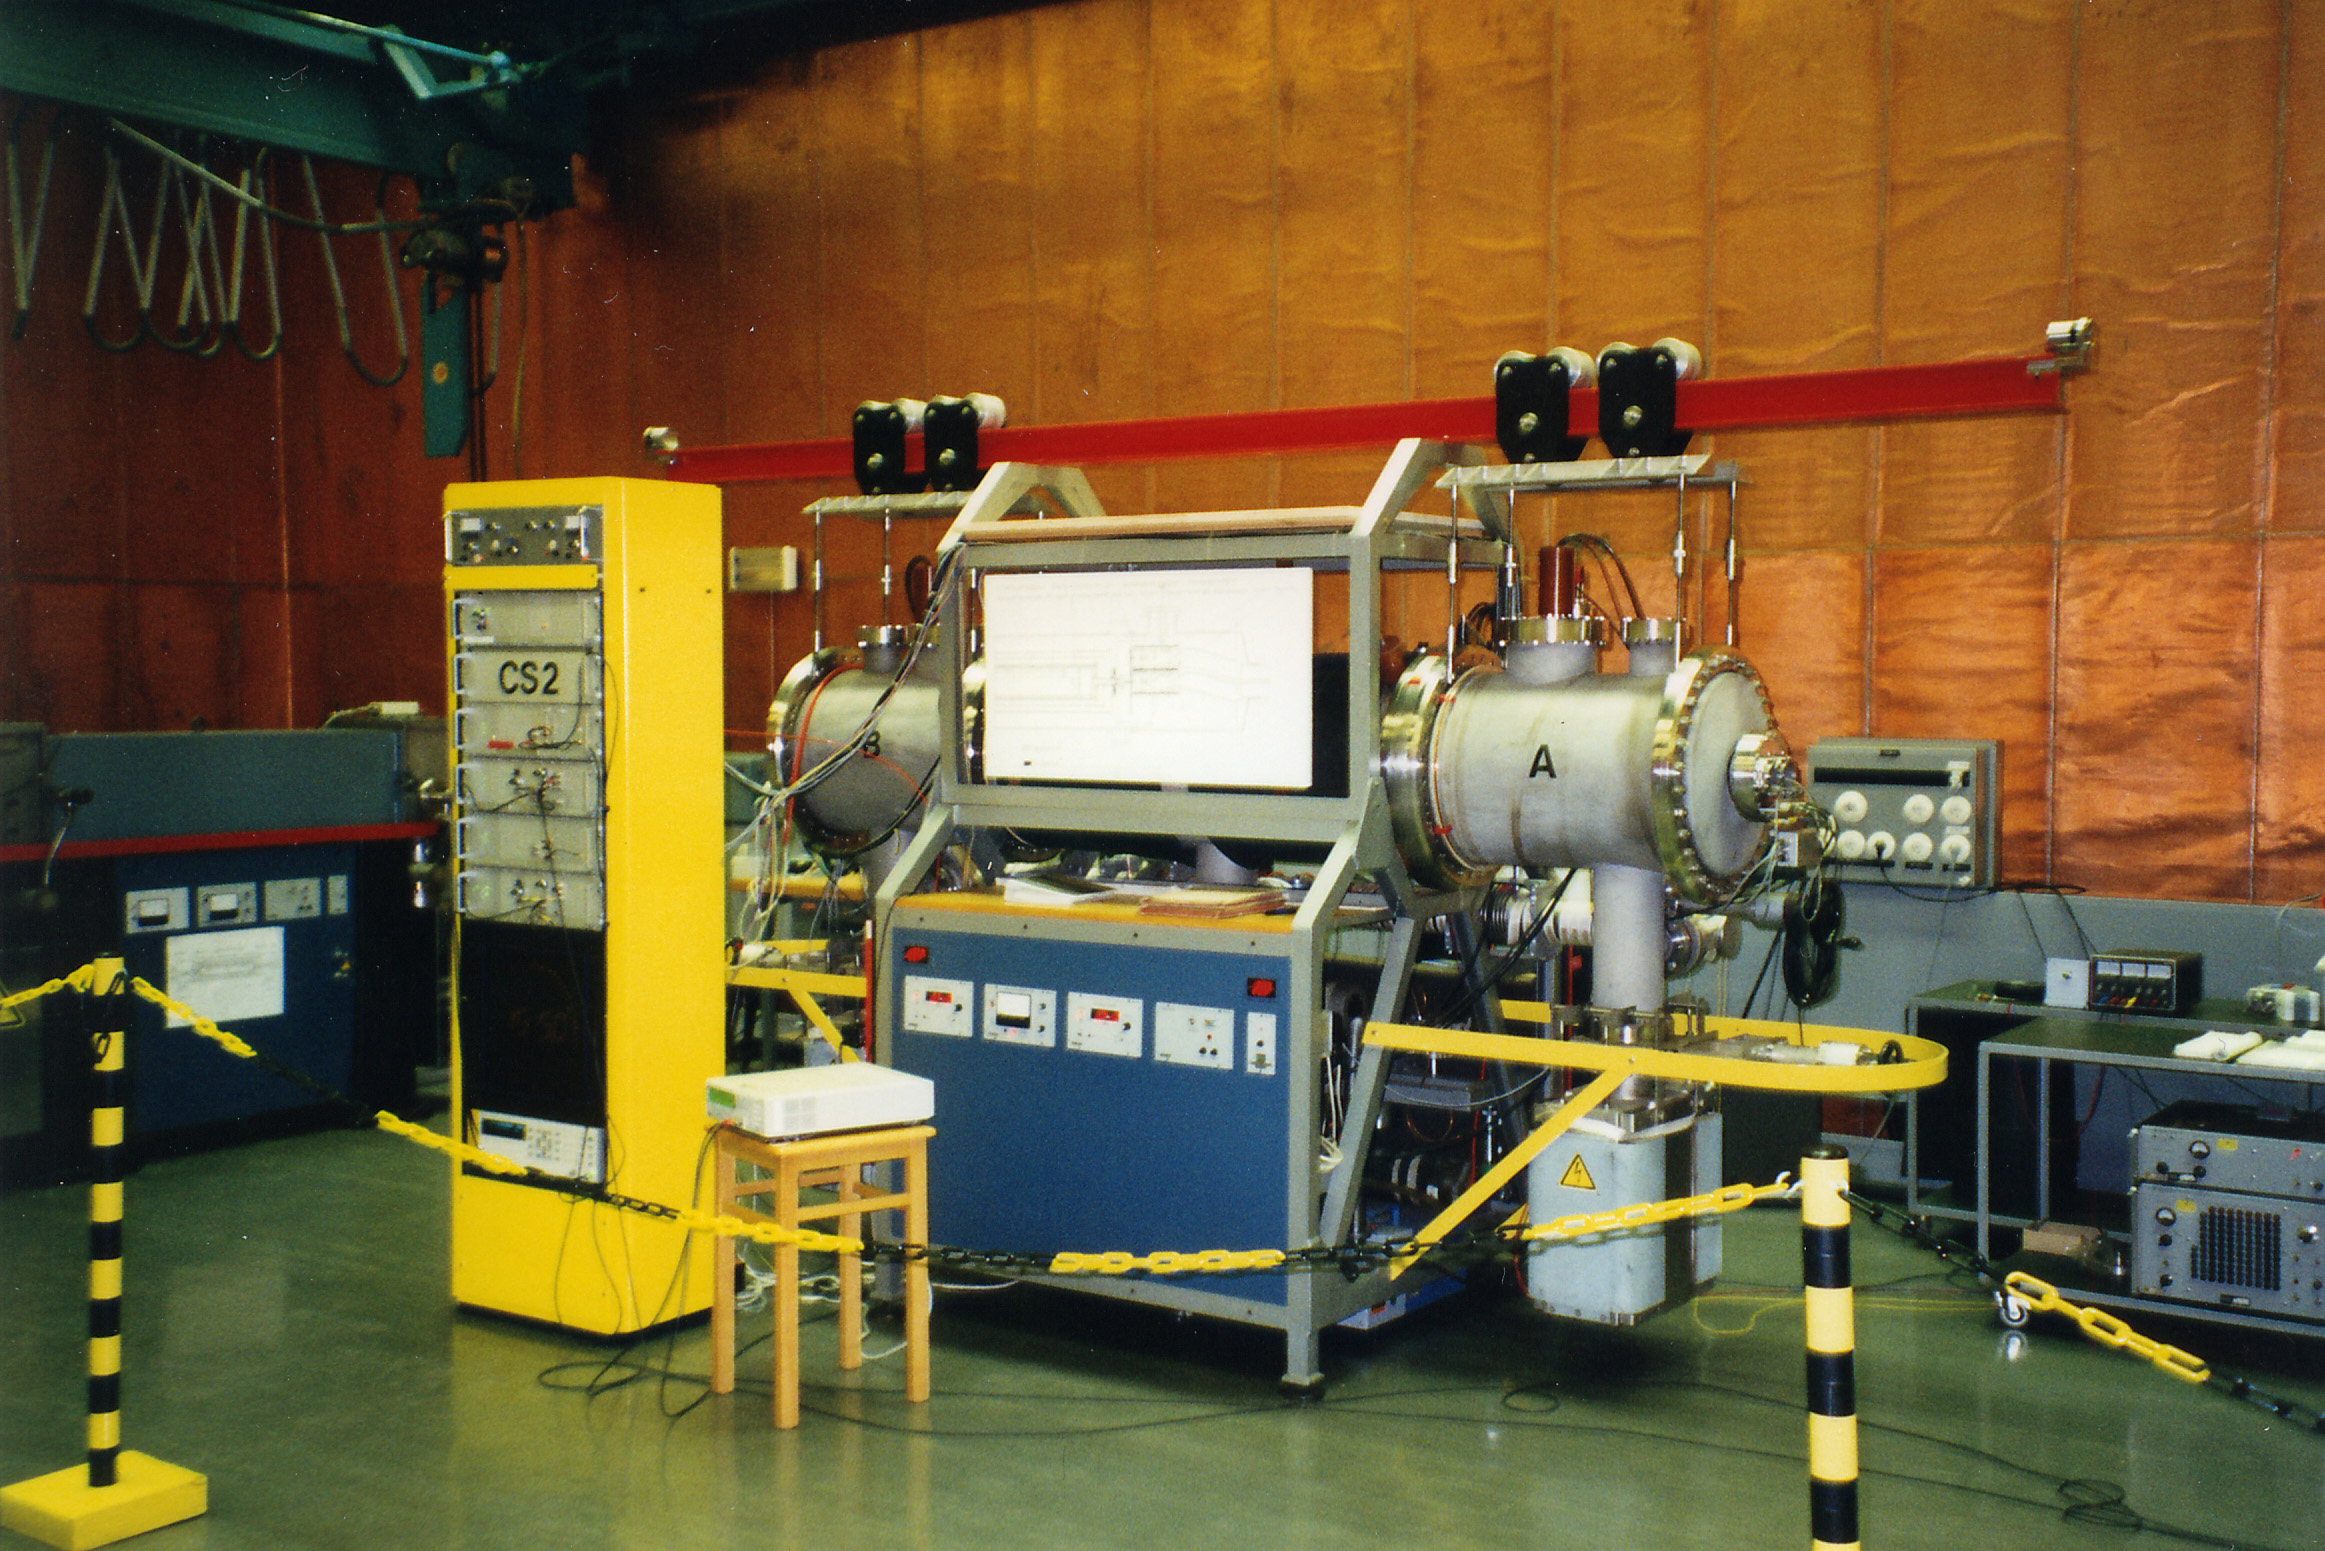
\includegraphics[height=3.5cm]{images/Atomuhr-CS2.jpg}\\[-1.2\baselineskip]
          \hspace{3.5cm}{\color{black!20}\small[Jörg Behrens]}
        \end{center}

        \begin{itemize}
          \item Based on clocks
          \item Monotonically ticking SI seconds
        \end{itemize}
      }
    \end{column}
  \end{columns}
  \medskip
  \begin{columns}[t, onlytextwidth]
    \begin{column}{0.475\textwidth}
      \onslide<2->{%
        \begin{center}
          \large\bfseries
          Measured daily by radio telescopes\\ (e.\,g.\ by the VLBA)
        \end{center}
      }
    \end{column}
    \hfill
    \begin{column}{0.525\textwidth}
      \onslide<4->{%
        \begin{center}
          \large\bfseries
          Measured by atomic clocks\\
        \end{center}
      }
    \end{column}
  \end{columns}
\end{frame}

\begin{frame}{Time Standards}
  \framesubtitle{UT1, ERA, TAI, TT}
  \begin{columns}[t, onlytextwidth]
    \begin{column}{0.495\textwidth}
      \begin{center}
        \heading{Earth's Orientation}

        \begin{description}[ERA $(\theta)$]
          \item[UT1] Universal Time 1
            \begin{itemize}
              \item Measured daily by VLBI
              \item Units have variable length, since $\SI{1}{\day} = \SI{24}{\hour} = \SI{1440}{\minute} = \SI{86400}{\second}$
              \item Can only be known in hindsight
              \item Published as $\increment(\operatorname{UT1}, \operatorname{UTC})$ tables
            \end{itemize}
          \item[ERA ($\theta$)] Earth Orientation Angle \\
            UT1 expressed as angle
        \end{description}
      \end{center}
    \end{column}
    \begin{column}{0.495\textwidth}
      \begin{center}
      \heading{Linear Time}
        \begin{description}[TAI]
          \item[TAI] Temps Atomique International
            \begin{itemize}
              \item Maintained by the BIPM
              \item Uses $>600$ atomic clocks in 60 institutes
              \item Preliminary \TAI{} time broadcast
              \item Final \TAI{} published monthly
              \item SI seconds on Earth's Geoid\\ → relativistic corrections
            \end{itemize}
          \item[TT] Terrestrial Time
            \begin{itemize}
              \item Idealised timescale for time on Earth's Geoid
              \item Realized as $\TT(\TAI) = \TAI{} + \SI{32.184}{\second}$
            \end{itemize}
        \end{description}
      \end{center}
    \end{column}
  \end{columns}
\end{frame}

\begin{frame}[c]{Time Standards}
  \framesubtitle{UTC}
  \begin{columns}[c, onlytextwidth]
    \begin{column}{0.5\textwidth}
      \centering
      \textbf{\Large Bit of Both}\\[0.5\baselineskip]%
      \begin{description}[UTC]
        \item[UTC] Coordinated Universal Time
        \begin{itemize}
          \item Civil Timekeeping
          \item Based on \TAI
          \item Difference to \UT{} kept $<\SI{1}{\second}$ by leapseconds \\
            \texttt{2020-12-31T23:59:60}
          \item Currently: $\UTC = \TAI - \SI{37}{\second}$
        \end{itemize}
      \end{description}
    \end{column}
    \hfill
    \begin{column}{0.5\textwidth}
      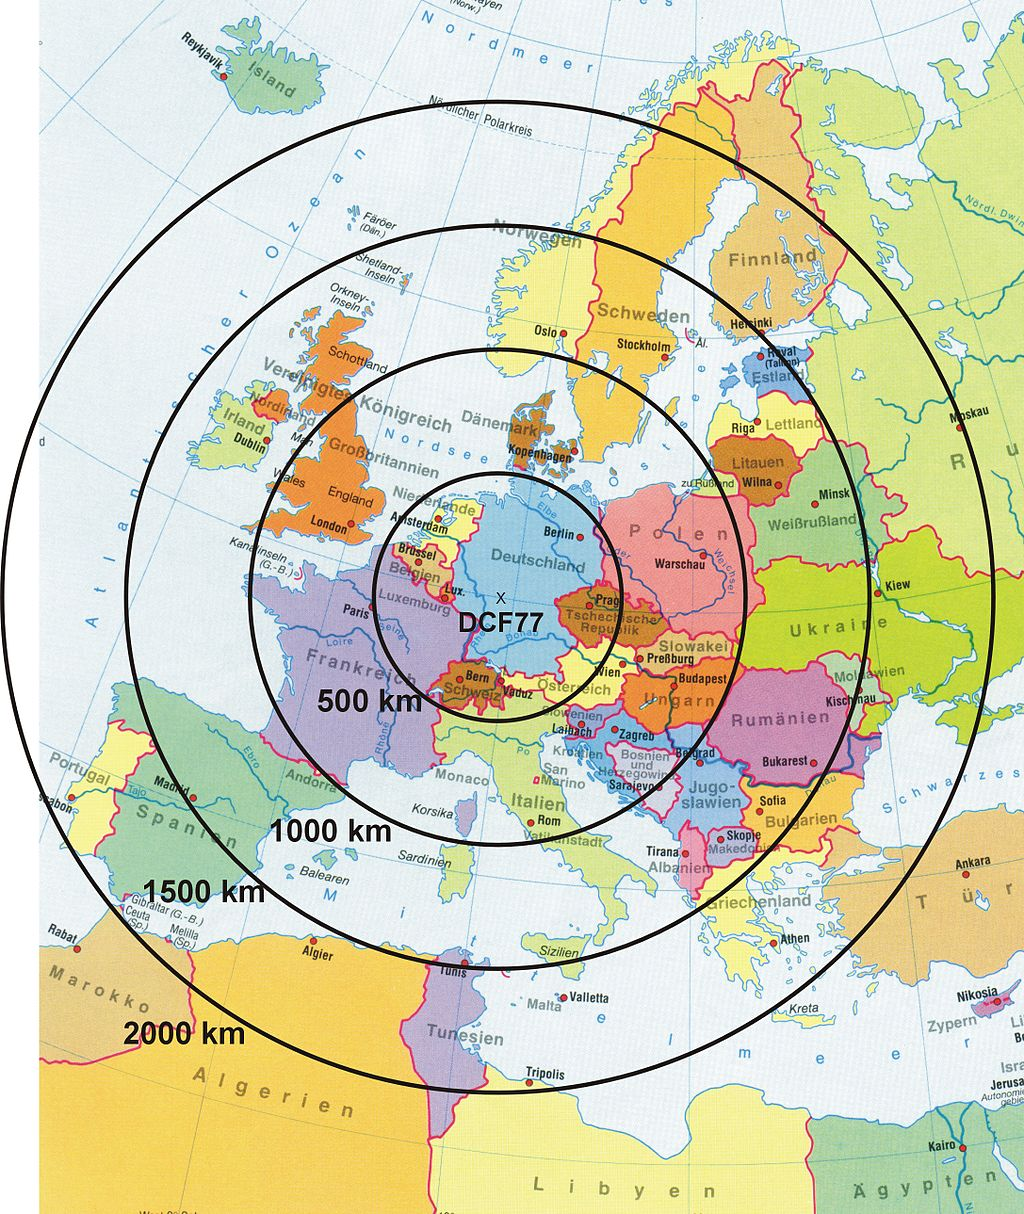
\includegraphics[height=0.9\textheight]{images/dcf77.jpg}\\[-1.2\baselineskip]
      \hspace{2em}[PTB (Erika Schow)]
    \end{column}
  \end{columns}
\end{frame}

\section{Terrestrial Coordinates}
\bumper{Terrestrial Coordinates}

\begin{frame}{International Terrestrial References System and Frames}

  The ITRS is defined by axis fixed on the Earth's crust with no net rotation
  through continental drift

  \begin{description}[$(0,0,0)$]
    \item[$\color{vertexDarkRed} z$-Axis] Earth's rotation axis
    \item[$\color{vertexDarkRed} x$-Axis] in the equatorial plane through the 0 meridian
    \item[$\color{vertexDarkRed} y$-Axis] perpendicular to $x$ and $z$ form a right handed system
    \item[$\color{vertexDarkRed} (0, 0, 0)$] Earth's barycenter
  \end{description}

  We mostly use spherical coordinates: latitude, longitude and height above
  the reference geoid.

  \bigskip

  A reference frame is an implementation of a reference system based on ground stations:

  \begin{itemize}
    \item GPS (Global Positioning System) / Galileo ground stations
    \item VLBI telescopes
    \item Satellite laser ranging
    \item DORIS (Doppler Orbitography and Radiopositioning Integrated by Satellite)
  \end{itemize}
\end{frame}

\begin{frame}[t]{ITRF / WGS84}
  \centering
  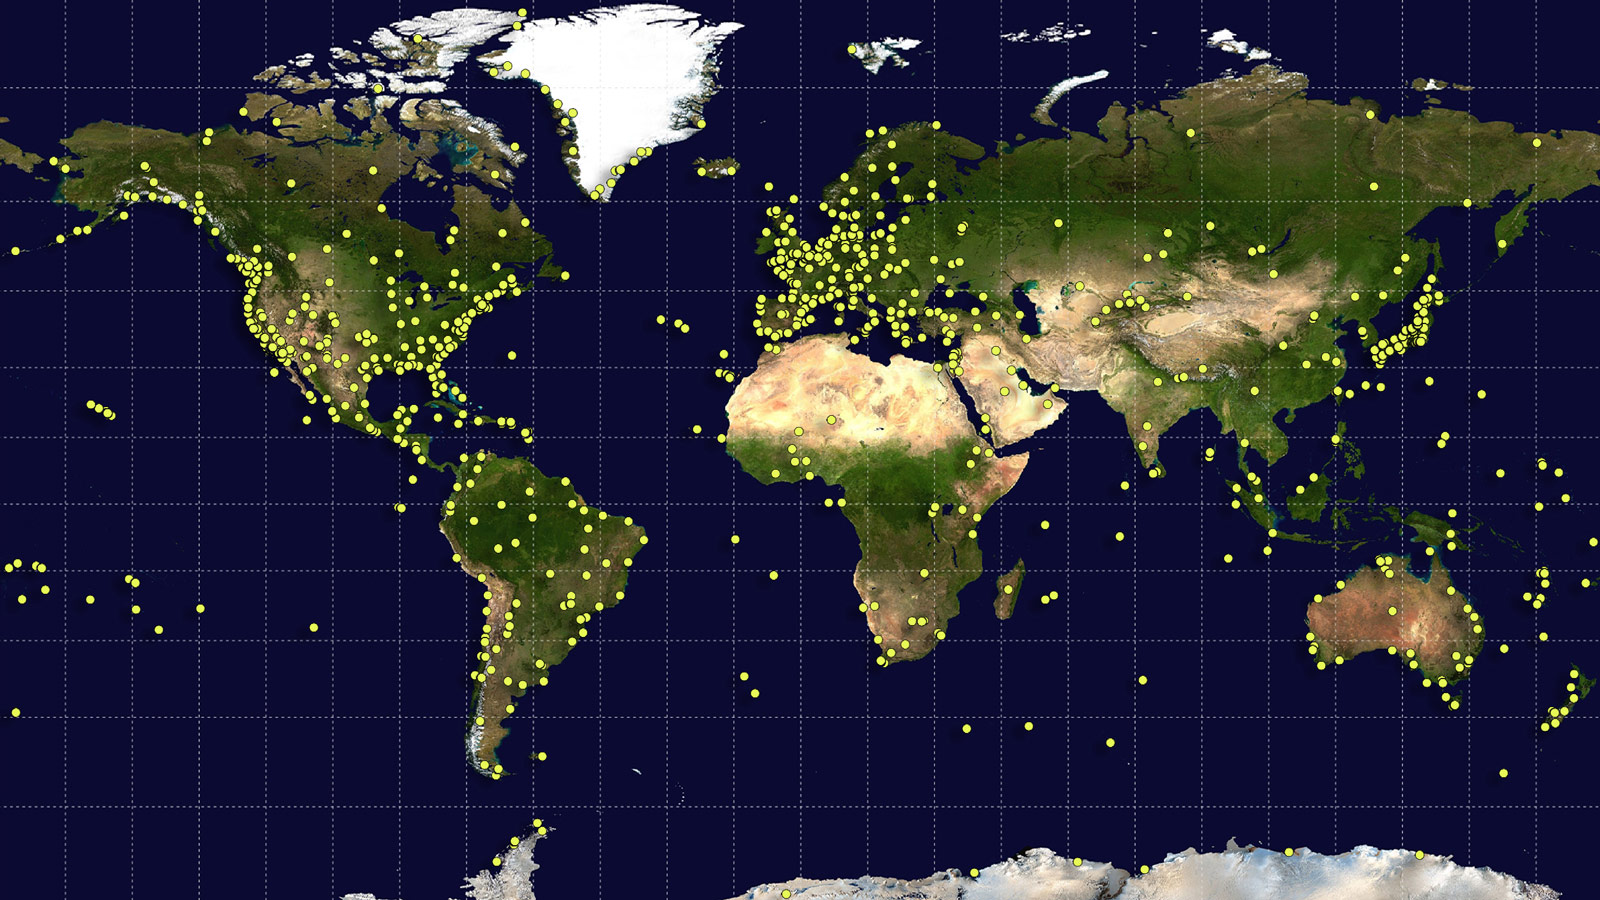
\includegraphics[
    width=\textwidth,
    height=0.9\textheight,
    keepaspectratio
  ]{images/itrf_groundstations.jpg}\\[-3\baselineskip]
  \textcolor{white}{[NASA/Earth Observatory/GSFC]}\\[2\baselineskip]

  Two main reference frames today: WGS84 and ITRF. Difference only centimeters.
\end{frame}

\section{Precession / Nutation / Polar Motion}
\bumper{Precession / Nutation / Polar Motion}

\begin{frame}{Earth's unstable axis of rotation}
  \begin{columns}[c, onlytextwidth]
    \begin{column}{0.5\textwidth}
      \begin{itemize}
        \item All solar system bodies apply a force onto Earth's rotation axis
        \item Division into two components
      \end{itemize}

      \bigskip

      \heading{Precession}
      \begin{itemize}
        \item Smooth, circular motion of the axis
        \item Period ca.\ ~26\,000 years
      \end{itemize}

      \bigskip
      \heading{Nutation}
      \begin{itemize}
        \item All other periodic components
        \item Current model: 678 terms for sun and moon, 687 terms for the planets
          $⇒$ \SI{0.3}{\micro\arcsecond} precision
      \end{itemize}

      \bigskip
      Precisions discarding Nutation:

      \medskip
      Without nutation: $\approx\ang{;;30}$ precision \\
      3rd order approximation: $\approx\ang{;;1}$ precision
    \end{column}
    \hfill
    \begin{column}{0.45\textwidth}
      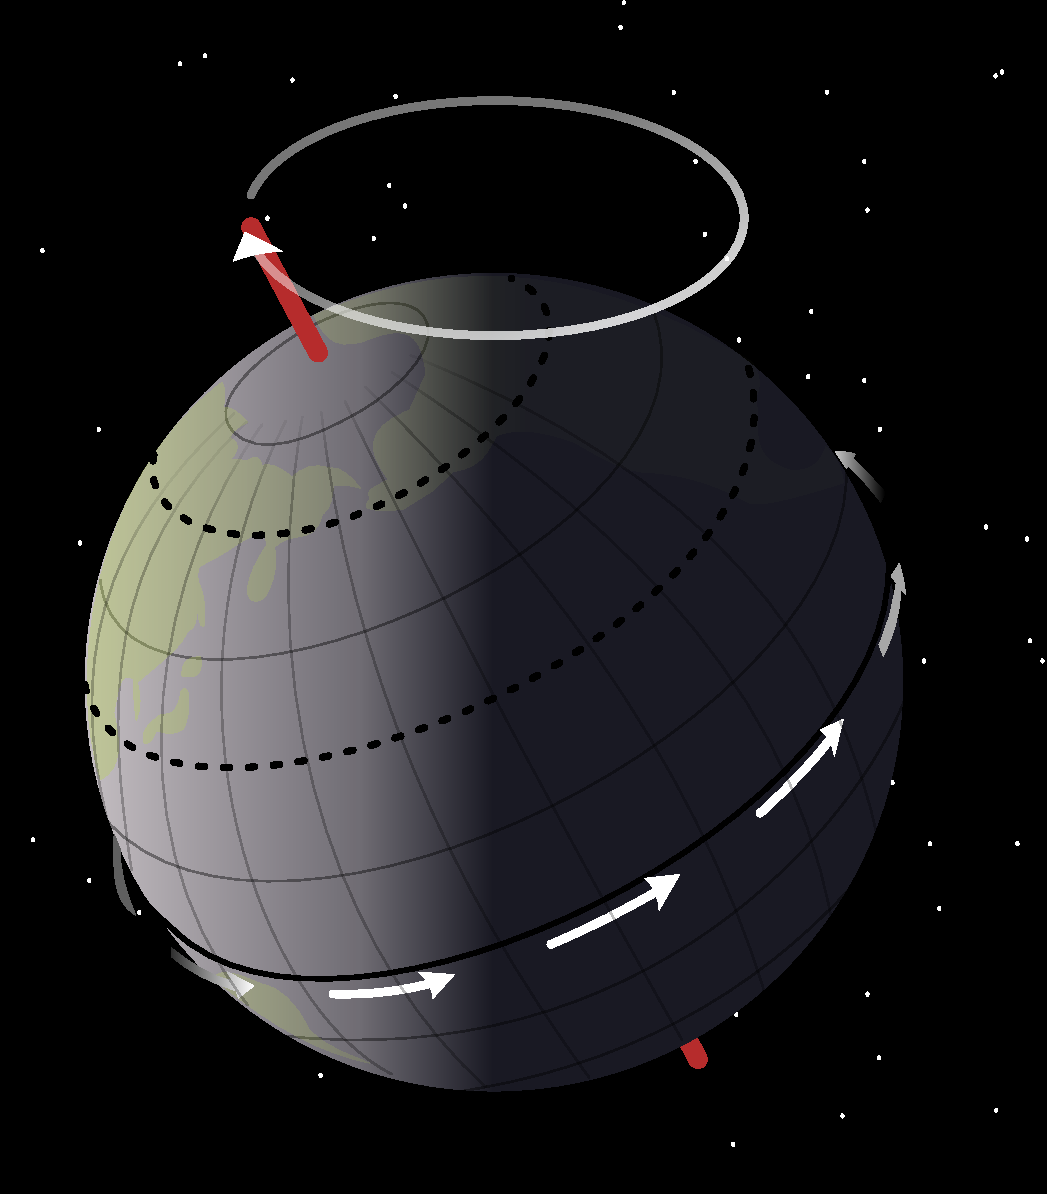
\includegraphics[width=\textwidth]{images/earth_precession.pdf}
    \end{column}
  \end{columns}
\end{frame}

\begin{frame}[c]{Polar Motion}
  \begin{columns}[c, onlytextwidth]
    \begin{column}{0.35\textwidth}
      \begin{itemize}
        \item Earth's rotation axis also not stable with respect to the crust
      \end{itemize}
    \end{column}
    \hfill
    \begin{column}{0.6\textwidth}
      \includegraphics[width=\textwidth]{build/polar_motion.pdf}
    \end{column}
  \end{columns}
\end{frame}

\begin{frame}[c]{Frame summary}
  \Huge
  \begin{equation*}
    \symbf{x}_\text{earth} = \underbrace{
      \symbf{W}^{-1} \cdot \symbf{T}^{-1} \cdot \underbrace{
        \symbf{N}^{-1} \cdot \symbf{P}^{-1} \cdot \underbrace{
          \symbf{x}_\text{sky}
        }_\text{ICRS}}_{\mathclap{\text{CIRS}}}}_\text{ITRF}
  \end{equation*}

  \large
  \begin{description}
    \item[$\symbf{P}$] Precession
    \item[$\symbf{N}$] Nutation
    \item[$\symbf{T}$] Earth's rotation
    \item[$\symbf{W}$] Polar Motion
  \end{description}
\end{frame}

\section{Horizontal Coordinates}

\begin{frame}{Horizontal Coordinates}


  \begin{columns}[c, onlytextwidth]
    \begin{column}{0.35\textwidth}
      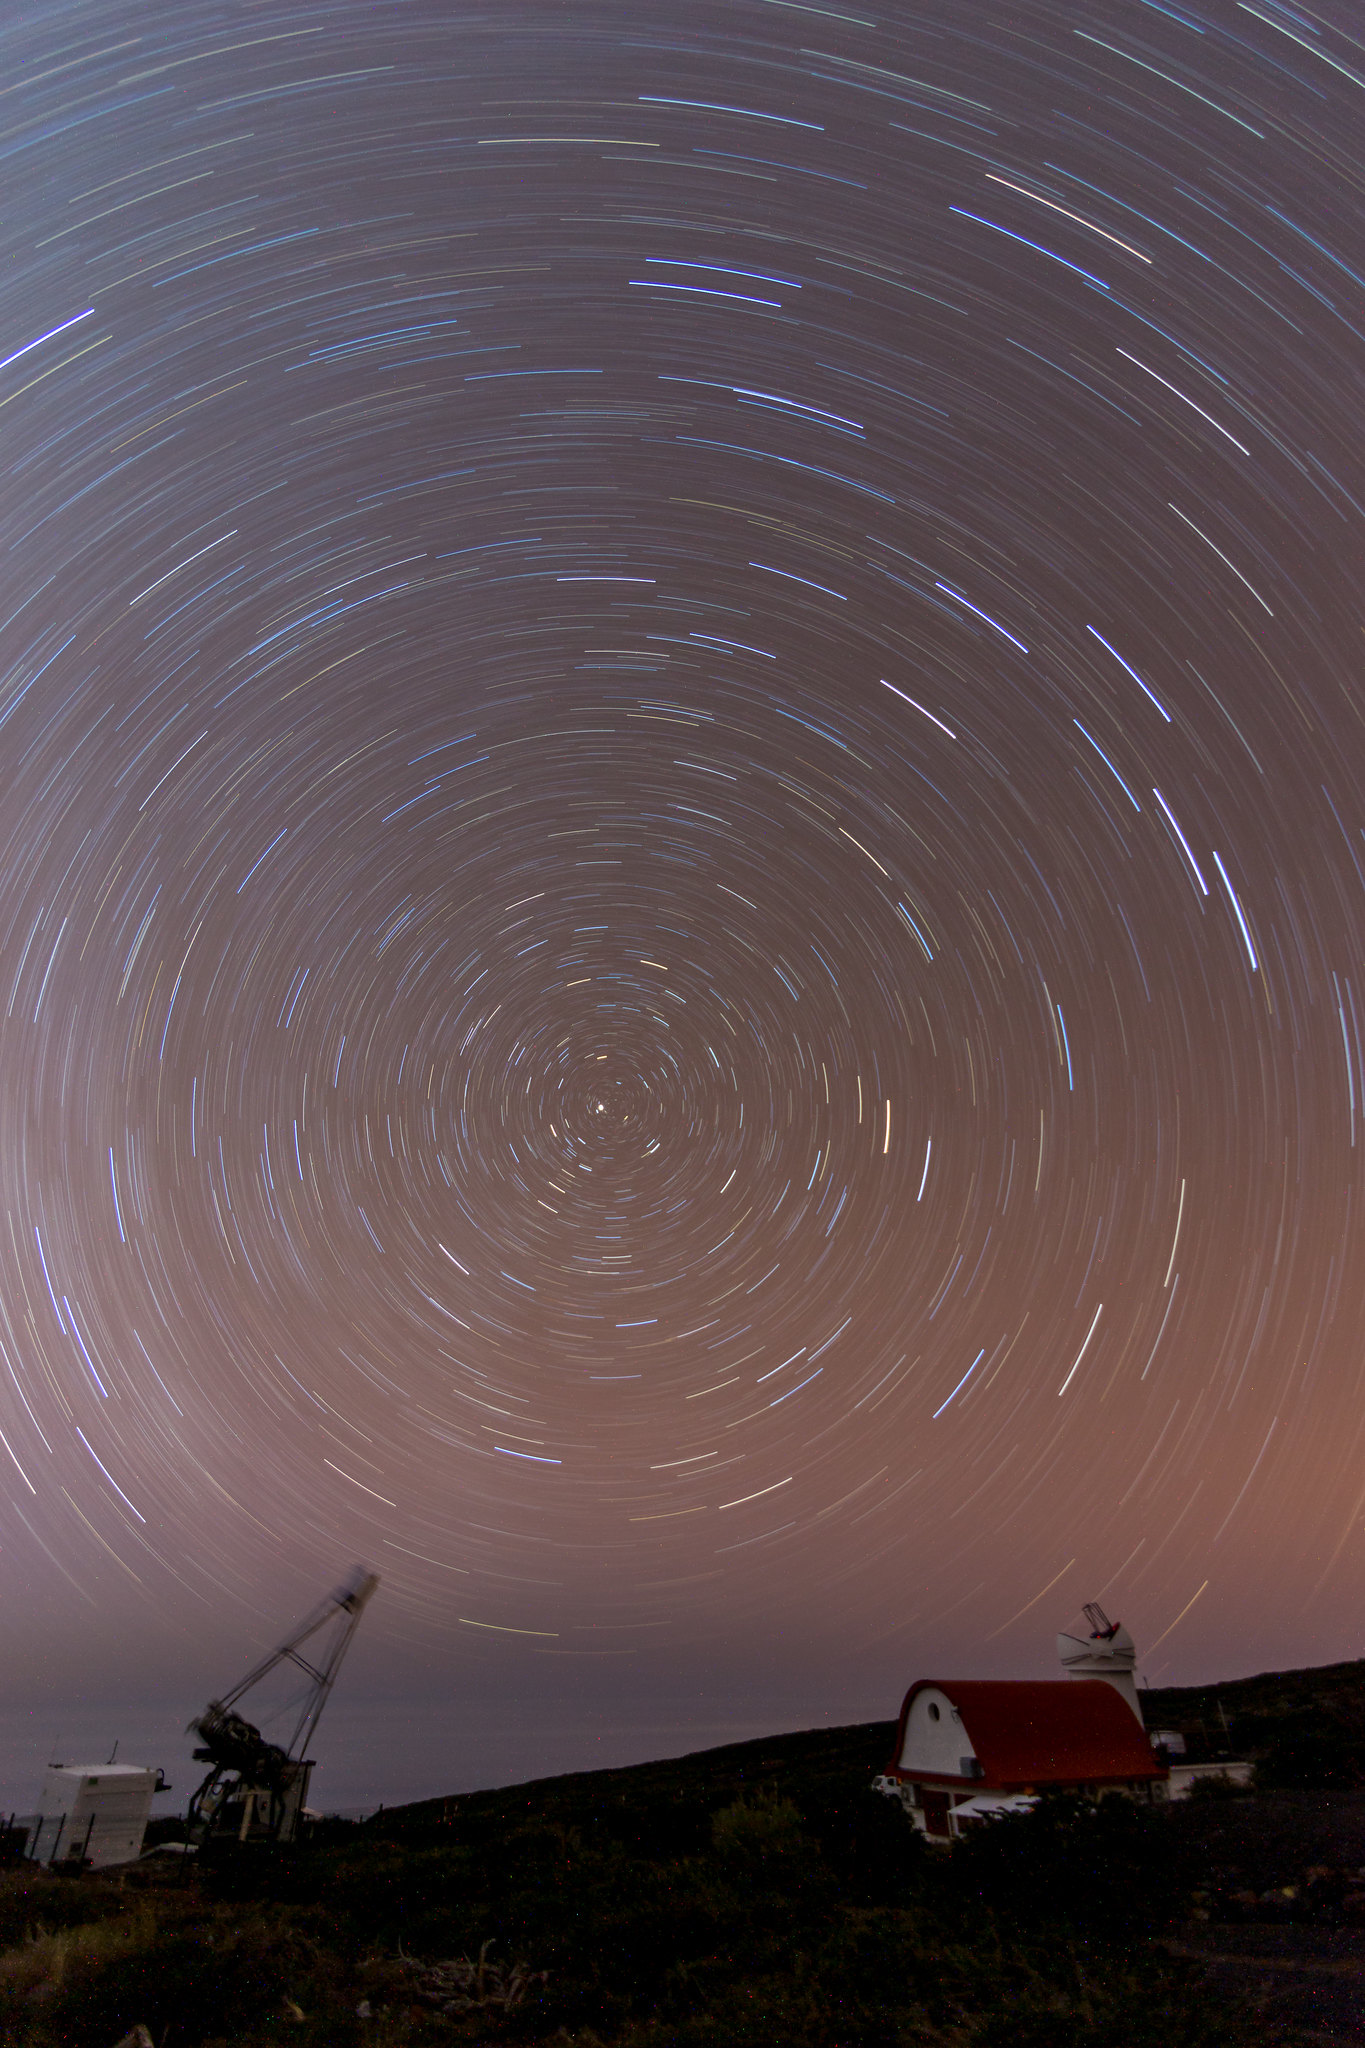
\includegraphics[width=\textwidth]{images/trails.jpg}
    \end{column}
    \hfill
    \begin{column}{0.6\textwidth}
      From the ITRF, we then got to a local coordinate system.

      \begin{itemize}
        \item Coordinate system for the local observer
        \item Several definitions exist
        \item astropy:
          \begin{description}
            \item[Altitude] Angle above the horizontal plane
            \item[Azimuth] Angle in the plane, N = \ang{0}, E = \ang{90}
            \item[Zenith] $\ang{90} - \text{Altitude}$
          \end{description}
      \end{itemize}
    \end{column}
  \end{columns}
\end{frame}

\begin{frame}{Things not mentioned today}
  \begin{itemize}
    \item Galactic coordinates (simple rotation from ICRS)
    \item Solar system bodies
    \item Refractive corrections
    \item All the old definitions still in use at many places \\
      (GMST, J2000 coordinates, Equation of the equinox, ...)
  \end{itemize}
\end{frame}

\section{Using \texttt{astropy} for Coordinate Transformation}
\bumper{Never do live demo}

\end{document}
